\documentclass{article}
\usepackage{amsmath}
\usepackage{graphicx}
\begin{document}
\author{Ana Bhattacharjee}
\title{Quiz 2: Question 35}
\date{\today}
\maketitle{}

\begin{center}
In order to find the center of the circle, we take the midpoint of each circumference terminal.
\begin{align}
M = (\frac{x_1 + x_2}{2}, \frac{y_1 + y_2}{2}) \\
M_{\circ} = (\frac{3 + 3}{2}, \frac{0 + (-7)}{2}) \\
M_{\circ} = (\frac{6}{2}, \frac{-7}{2}) \rightarrow (3, -\frac{7}{2})
\end{align}

Now that we have the midpoint of the diameter, we now also have the center of the circle represented as the coordinate (h,k). We now need to take the distance of the midpoint to any of the circumference endpoints to get the radius's length.
\par
\begin{align}
  d = \sqrt{(x_2 - x_1)^2 + (y_2 - y_1)^2} \\
  d = \sqrt{(3 - 3)^2 + (\frac{-7}{2} - 0)^2} \rightarrow \sqrt{0 + \frac{49}{4}} = \frac{7}{2} \\
  d = r \\
  r = \frac{7}{2}
\end{align}
The equation of a circle in standard form is represented as $ (x - h)^2 + (y - k)^2 = r^2 $ so the equivalent format for this problem is:
\begin{align}
  (x - 3)^2 + (y + \frac{7}{2})^2 = \frac{49}{4}
\end{align}
\par
The circle is plotted below.
\begin{figure}[!htbp]
  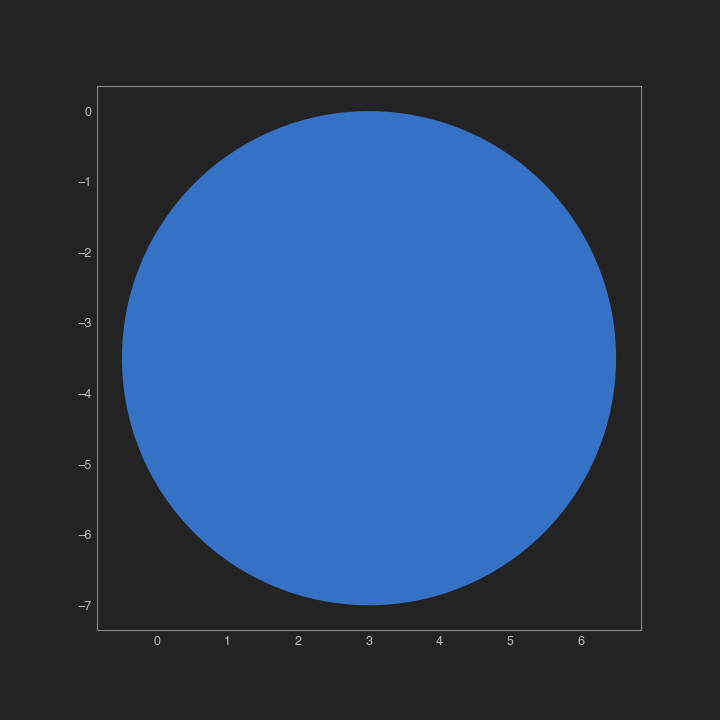
\includegraphics[width=1\columnwidth]{../q35/circle}
  \caption{Circle in Graphical Form}
\end{figure}
\end{center}

\end{document}
